
\chapter{Improvements}


\label{seq:thenew}

Using the analysis carried out in the previous chapters, we suggest  improvements to the existing methods of focal length computing.

\section{f-Ratio}
We present and analyze the performance of a new algorithm, called f-Ratio, for robust focal lengths computation. The algorithm uses the premise that the ratio of focal lengths is more robust to achieve superior accuracy. The algorithm serves as a further proof that explicitly using the ratio of the focal lengths may by beneficial for the performance.

\subsection{Algorithm}

The idea of the algorithm is to use a new solver that would compute $\mathtt{F}$ from 6 correspondences given the ratio $r=f_2 \slash f_1$. We create such a solver using the automatic generator~\cite{generator}. The solver uses the Demazure polynomials, i.e.\ the rank and the constraints~\ref{eq:rank},~\ref{eq:trace} in terms of elements of the matrix $\mathtt{F}$, $f_1$, and $r$. 

 A solver assuming fixed focal length $f_1=f_2$ could be used instead, for example that of Torii et el.~\cite{Aki6pt}, by first rescaling \[\V{x}_2^{r}= \mat{ccc}{r & 0 & 0 \\ 0 & r & 0 \\ 0 & 0 & 1} \V{x}_2.\] The output of such solver would be $f_1$ and $\mathtt{F}$. We can compute $f_2$ as $f_1  r$.  

Both solvers give same results up to machine precision. Both solvers also yield 15 (possibly non-real) solutions. 

\begin{algorithm}[H]
\SetAlgoNoLine
\LinesNotNumbered
\KwData{A list of 7 right image points $\V{x}_1$ and a list of the corresponding left image points $\V{x}_2$, lists of remaining tentative correspondences $\V{x}_1^{test}, \V{x}_2^{test}$, 6pt solver $solve6pt$}
\KwResult{Fundamental matrix $F$}
 \Begin
    {Estimate $\M{F}_0$ from all correspondences\;
    
    Estimate $r=f_2 \slash f_1$ from $\M{F}_0$ \;
    
    \ForEach{6-tuple $\V{x}_1^6$ of points drawn from $\V{x}_1$} 
        {
        $\V{x}_2^6 \leftarrow$ corresponding points to $\V{x}_1^6$ from $\V{x}_2$ \;
        $\M{F}s_i \leftarrow solve6pt(\V{x}_1^6,\V{x}_2^6,r)$\;
        $\M{F}_i \leftarrow$ the matrix from $ \M{F}s_i$ which best explains $\V{x}_1^{test}, \V{x}_2^{test}$,
        }
        
    \Return{$F_i$ which best explains $\V{x}_1^{test}, \V{x}_2^{test}$}
    }
 \caption{f-Ratio}
 \label{f-Ratio}
\end{algorithm}

The solver needs to compute and test 7 $\times$ 15 fundamental matrices\footnote{At most. The 6pt solver usually gives from 9 to 14 real solution, but the maximal possible number is 15. }, which still may be bearable time for a RANSAC-based method. 

One may construct a version of the algorithm which works with all the available points, however,  in such an algorithm one would need to test a combinatorially growing number of matrices.
%\footnote{At most. The 6pt solver usually gives from 9 to 14 real solution, but the maximal possible number is 15. }
%, the amount of computation needed is much bigger. 

\subsection{Performance}

We assess the performance of the algorithm in a similar manner as in the previous analysis. Fig.~\ref{fratio_nonoise} a comparison our f-Ratio method and the baseline 7pt algorithm. 

\begin{figure}[h!]
  \begin{center}
    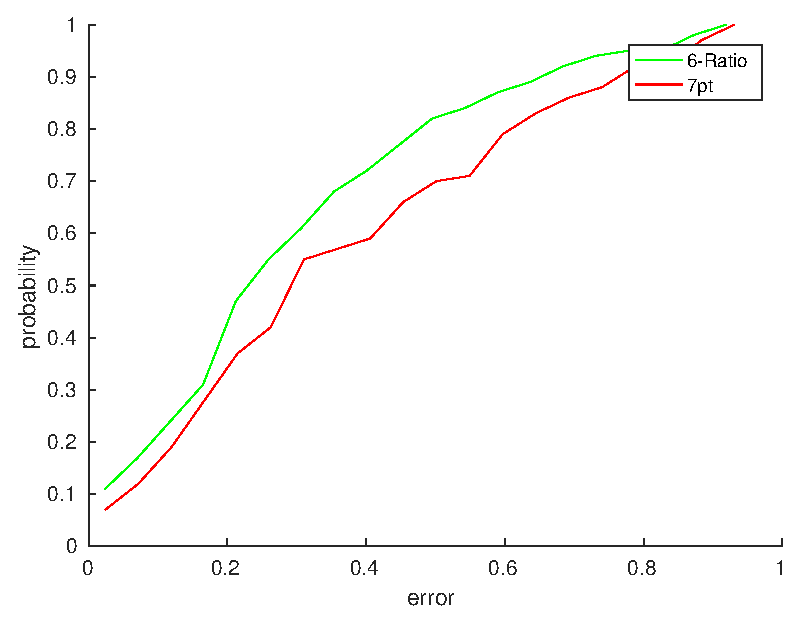
\includegraphics[width=\linewidth]{ratio6_nonoise.eps}
    \caption[Performance of f-Ratio]{A comparison of 6-Ratio against the baseline. The cumulative distribution of the  multiplicative error (equation \ref{eq:error})  in the focal  length  estimates is shown.}
    \label{fratio_nonoise}
  \end{center}
\end{figure}

In the next experiment, Fig.~\ref{fratio_10noise} we add an additional amount of noise ($\sigma=10$ pixels) to one of the points. This demonstrates that our method can cope with outliers even better than the standard RANSAC algorithm.

\begin{figure}[h!]
  \begin{center}
    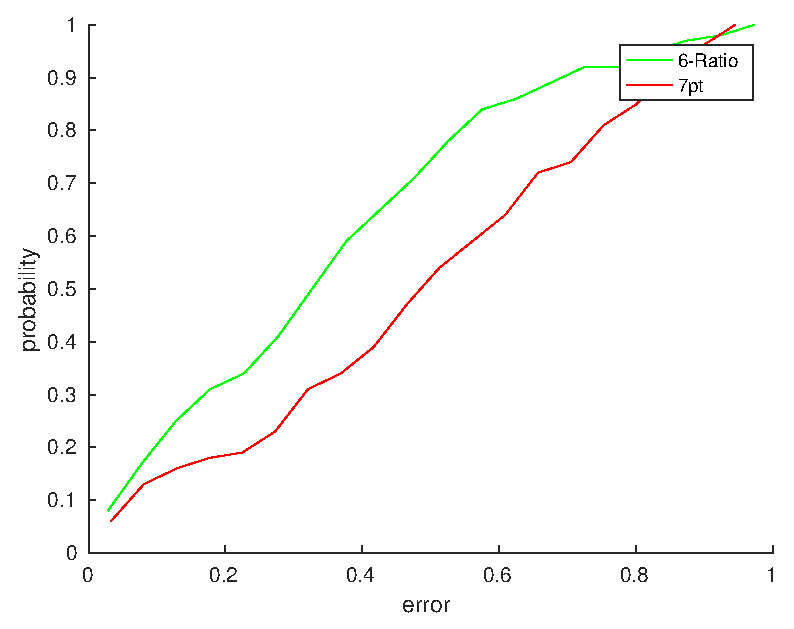
\includegraphics[width=\linewidth]{ratio6_10noise.eps}
    \caption[Performance of f-Ratio with one outlier]{A comparison of 6-Ratio against the baseline in presence of outliers. The cumulative distribution of the  multiplicative error (equation \ref{eq:error})  in the focal  length  estimates is shown. }
    \label{fratio_10noise}
  \end{center}
\end{figure}

The results show that it is possible to reconstruct  scenes better with f-Ratio than with 7pt algorithm. The algorithm  \ref{f-Ratio} successfully demonstrates that explicitly using estimated ratio of focal lengths
%over the focal lengths themselves
may improve the accuracy of the estimation.

\section{Prior focal length}

Hartley~\cite{HartleyPriors} describes an iterative algorithm for computing focal lengths from point correspondences, which incorporates prior information about focal lengths and principal points. The algorithm uses a Levenberg-Marquardt optimization. In this section we describe an improvement to his algorithm. Using computed focal length ratio $r=f_2 \slash f_1$, we are able to get better focal lengths estimates.

\subsection{Original Hartley's algorithm}

Original Hartley's algorithm optimizes a certain cost function given the weights $w_i$, point correspondences $\mathtt{x}_1$, $\mathtt{x}_2$, prior focal length  $\bar{f}_1$, $\bar{f}_2$, minimal focal length $f_{min}$ and prior principal points $\bar{\mathbf{p}}_1$, $\bar{\mathbf{p}}_2$. We give this cost function as algorithm \ref{alg:hart_cost}. 


Note that the focal lengths are not in the list of the parameters to this cost function, as they are determined by the fundamental matrix and principal points.

\begin{algorithm}
\SetAlgoLined 
\LinesNotNumbered
 \KwData{Fundamental matrix $\mathtt{F}$, principal points $\mathbf{p}_1$, $\mathbf{p}_2$.}
 \KwResult{Vector of costs (errors) $\mathbf{C}$}
 \Begin
    {From $\mathtt{F}$, $\mathbf{p}_1$, $\mathbf{p}_2$ compute $f_1$, $f_2$\;
    
    $C_\mathtt{F} \leftarrow$ Sampson error of the matrix $\mathtt{F}$ on the points $\mathtt{x}_1$, $\mathtt{x}_2$\;
    
    
    $C_f \leftarrow w_1^2(f_1^2-\bar{f}_1^2)^2 + w_2^2(f_2^2-\bar{f}_2^2)^2  + w_d^2(f_1^2-f_2^2)^2 + w_{z1}^2(f_{min}^2 - f_1^2)^2 + w_{z2}^2(f_{min}^2-f_2^2)^2 $\;
    
    $C_\mathbf{p} \leftarrow w_p^2 \norm{\mathbf{p}_1-\bar{\mathbf{p}}_1}^2 + w_p^2 \norm{\mathbf{p}_2-\bar{\mathbf{p}}_2}$\;
    
    \Return{Costs $C_\mathtt{F}$, $C_\mathbf{p}$, $C_f$\;}}
 \caption{The cost function of Hartley~\cite{HartleyPriors}}
 \label{alg:hart_cost}
\end{algorithm}


The cost function of focal lengths $C_f$ incorporates a few interesting ideas besides using prior knowledge in first two terms. Its third term drives the focal lengths to the same value, which probably reflects the fact that most real cameras have similar focal lengths from a relatively small (compared to infinity) range. Also using such a term, the method should perform accurately even if the cameras used were indeed the same camera. The fourth and the fifth terms serve two purposes. Firstly, they prevent the squared focal lengths $f_1^2$, $f_2^2$ from becoming negative, which addresses the problem of imaginary focal lengths estimates. Secondly, these terms also prevent focal lengths from converging to zero. % Can this really happen when using Sampson error instead of x2 F x1 error?

Hartley suggests initializing the optimization with a technique he calls calibrated reconstruction, which is described as algorithm~\ref{alg:calrec}. The algorithm takes point correspondences and prior information about camera calibration, and returns a matrix which is consistent with priors. Hartley also claims that the returned matrix has small Sampson error on the point correspondences.

\begin{algorithm}
\SetAlgoLined 
\LinesNotNumbered
 \KwData{Point correspondences $\V{x}_1$, $\V{x}_2$, prior focal lengths $\bar{f}_1$, $\bar{f}_2$,prior principal points $\bar{\V{p}}_1$,$\bar{\V{p}}_2$.}
 \KwResult{Fundamental matrix $\M{F'}$}
 \Begin
    {Compute a fundamental matrix $\M{F}$ from point correspondences $\V{x}_1$, $\V{x}_2$ using the 7pt algorithm\;
    
    Create the prior calibration matrices $\bar{\M{K}}_1$, $\bar{\M{K}}_2$ from the $\bar{f}_1$, $\bar{f}_2$, $\bar{\V{p}}_1$,$\bar{\V{p}}_2$\; 
    
    Create an estimate of the essential matrix $\bar{\M{E}} = \bar{\M{K}}_2^T \M{F} \bar{\M{K}}_1$\;
    
    Compute $(\M{U}, \M{S}, \M{V}) = \text{svd} (\bar{\M{E}})$\;
    
    Take the two biggest singular values $s_1$, $s_2$
    Create an essential matrix $\M{E} = \M{U} \; \diag(\mat{ccc}{s_1 & s_2 & 0}) \; \M{V}$\;
    
    Create  a fundamental matrix which is consistent with the priors $\M{F}' =  \bar{\M{K}}_2^{-\T} \M{E} \bar{\M{K}}_1^{-1}$\;

    \Return{$\M{F}'$\;}
    }
 \caption{Calibrated reconstruction~\cite{HartleyPriors}}
 \label{alg:calrec}
\end{algorithm}


\subsection{Using ratio}

We introduce a modification based on use of estimated ratio of focal lengths $r= f_2\slash f_1$.  Given the correspondences, we use 7pt algorithm \ref{7pt} and the Bougnoux formula to estimate the ratio. We include the estimated ratio in cost function on $f$ from the function \ref{alg:hart_cost}: \[ C_f = w_1^2(f_1^2-\bar{f}_1^2)^2 + w_2^2(f_2^2-\bar{f}_2^2)^2  + w_d^2((r f_1)^2-f_2^2)^2 + w_{z1}^2(f_{min}^2 - f_1^2)^2 + w_{z2}^2(f_{min}^2-f_2^2)^2. \]

We show that such enhanced solver produces better focal length estimates. The graph \ref{hartley_ratio} shows the experiment with 100 runs of each solver.

\begin{figure}
  \begin{center}
    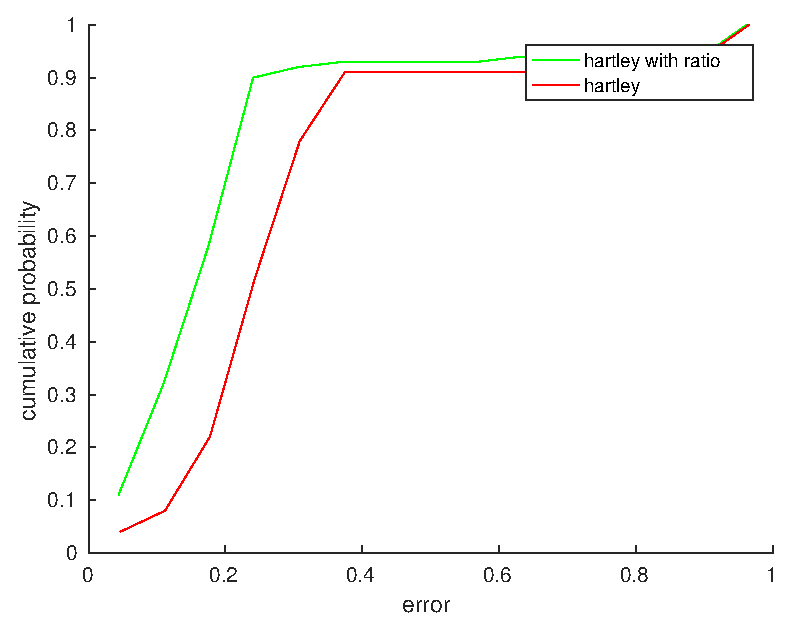
\includegraphics[width=\linewidth]{hartley_ratio_error.eps}
    \caption[Performance of Hartley solver with or without using ratio]{A comparsion of the Hartley algorithm~\cite{HartleyPriors} against our modified version which explicitly uses the ratio of the focal lengths $r = f_2 \slash f_1$ .  The cumulative distribution  of the  multiplicative error (equation \ref{eq:error})  in the focal  length  estimates.  The ground truth focal lengths were $(3,4)$. The prior focal lengths  were  drawn from an uniform distribution between $(3,4)$ and $(4.5, 5.5)$. The ground truth principal points were zero, and the prior principal points were $(0.1, 0.1)$. The number of correspondences used was 40, and the level of noise $\sigma$ was equal to 1. The weights on principal point priors were 10 times smaller than weights on focal lengths priors. }
    \label{hartley_ratio}
  \end{center}
\end{figure}

\subsection{Comparison of focal length computing methods}

We summarize the performance of several methods for estimating the focal lengths from the point correspondences. Besides previously mentioned, we use a method similar to the one from~\cite{Chandraker}. The method derived in the work is described as the algorithm~\ref{alg:Chandraker}

\begin{algorithm}[H]
\SetAlgoLined 
\LinesNotNumbered
 \KwData{Weights $w_i$, point correspondences $\mathtt{x}_1$, $\mathtt{x}_2$, prior focal length  $\bar{f}_1$, $\bar{f}_2$, prior principal points $\bar{\mathbf{p}}_1$, $\bar{\mathbf{p}}_2$.}
 \KwResult{Vector of costs (errors) $\mathbf{C}$}
 \Begin
    {Estimate the fundamental matrix $\mathtt{F}$ using the 7pt algorithm\;
    
    Define $p_1(f_1, f_2, \V{p}_1,\V{p}_2), p_2(f_1, f_2, \V{p}_1,\V{p}_2), p_3(f_1, f_2, \V{p}_1,\V{p}_2)$ as Kruppa equations~\cite{HartZiss}, rewritten as polynomials (see the paper~\cite{Chandraker})\;
    
    Minimize the following cost function:
    \begin{align*}
    %\label{eq:Chandraker}
    & f_1^*, f_2^*, \V{p}_1^*,\V{p}_2^* = & \\ = & \min_{f_1, f_2, \V{p}_1, \V{p}_2, \lambda_1, \lambda_2, \lambda_3} & w_1^2 (f_1 - \bar{f}_1)^2 + w_2^2 (f_2 - \bar{f}_2)^2  + w_p^2 \norm{\mathbf{p}_1-\bar{\mathbf{p}}_1}^2 + w_p^2 \norm{\mathbf{p}_2-\bar{\mathbf{p}}_2} \\ & \text{such that } & \lambda_1 p_1(f_1, f_2, \V{p}_1,\V{p}_2)+ \lambda_2 p_2(f_1, f_2, \V{p}_1,\V{p}_2) + \lambda_3 p_3(f_1, f_2, \V{p}_1,\V{p}_2)
    \end{align*}

    \Return{focal lengths $f_1, f_2$, principal points $\V{p}_1,\V{p}_2$\;}
    }
 \caption{The algorithm of Chandraker~\cite{Chandraker}}
 \label{alg:Chandraker}
\end{algorithm}

Note that the algorithm~\ref{alg:Chandraker}, contrary to the algorithm~\ref{alg:hart_cost} of Hartley, does not  change the fundamental matrix during the optimization. Instead, it computes the fundamental matrix beforehand, and the optimization finds a suitable combination of principal points and focal lengths that would be consistent with the fundamental matrix..

We use an optimization procedure obtained in private conversation to do the optimization in the last step of the algorithm~\ref{alg:Chandraker}.

The figures~\ref{opt_comp_f1}, \ref{opt_comp_f2} show the distribution of focal length as computed by different methods against different levels of noise in prior focal lengths. The distribution for each case is depicted using MATLAB function boxplot which shows 25$\%$ to 75$\%$ quantile values as boxes with a horizontal line for median. The crosses show data beyond 1.5 times the interquartile range. We use high level of noise ($\sigma$ = 4 pixels) to show that the regularization by priors allows us to handle bigger amount of noise. For smaller amounts noise  the difference between the Bougnoux formula and prior methods is not as pronounced.

We can observe in the figures~\ref{opt_comp_f1}, \ref{opt_comp_f2} that different methods behave inherently in a different way. The bougnoux formula has the biggest standard deviation of all, generally is noisy and gives a lot of outliers. The formula is also much less biased, and, of course, is independent of the given prior. The method of Hartley, because of the chosen cost function, tends to drive the focal lengths close to each other. Thus, it overestimates the smaller focal length in the Fig.~\ref{opt_comp_f1} and underestimates the bigger focal length in the Fig.~\ref{opt_comp_f1}. Our modified version of Hartleys' algorithm, as well as the method of Chandraker does not suffer from this. The algorithm of Chandraker apparently shows smaller standard deviation and is less influenced by the prior. 

\begin{figure}[h!]
  \begin{center}
    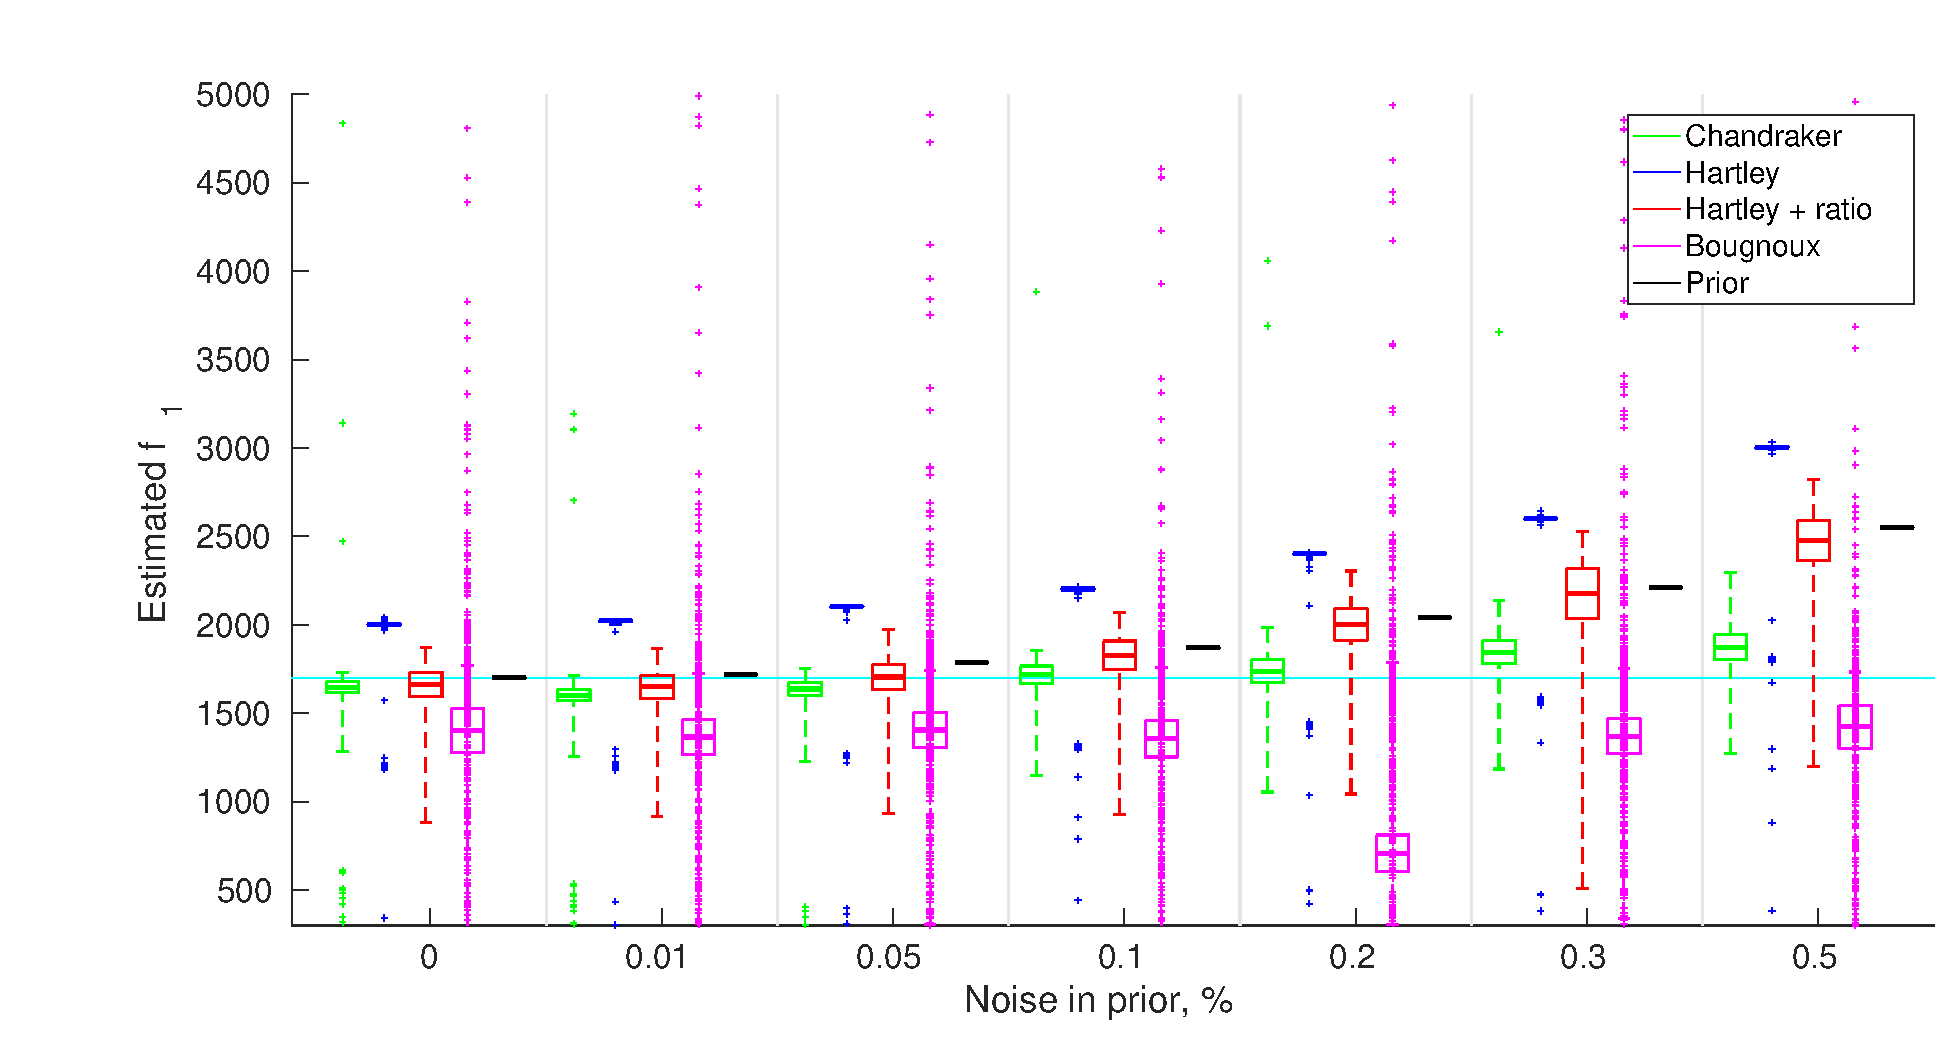
\includegraphics[width=\linewidth]{opt_comp_f1.eps}
    \caption[Comparison of the focal length methods. f1]{A comparison of the methods for computing focal lengths from point correspondences.  The ground truth focal length $f_1$ was 1700 (shown in cyan), and the relative noise (axis $x$) was added to it to produce priors, i. e., the priors were: 1700, 1717, 1785, 1870, 2040, 2210, 2550.  The ground truth principal points were both (10,20), and the prior principal points were $(0, 0)$. The number of correspondences used was 7, and the level of noise $\sigma$ was equal to 1. The weights on principal point priors were 10 times smaller than weights on focal lengths priors. The term enforcing the ratio of focal length in our modified version has the same weight as the terms for the focal lengths themselves.}
    \label{opt_comp_f1}
  \end{center}
\end{figure}



\begin{figure}[h!]
  \begin{center}
    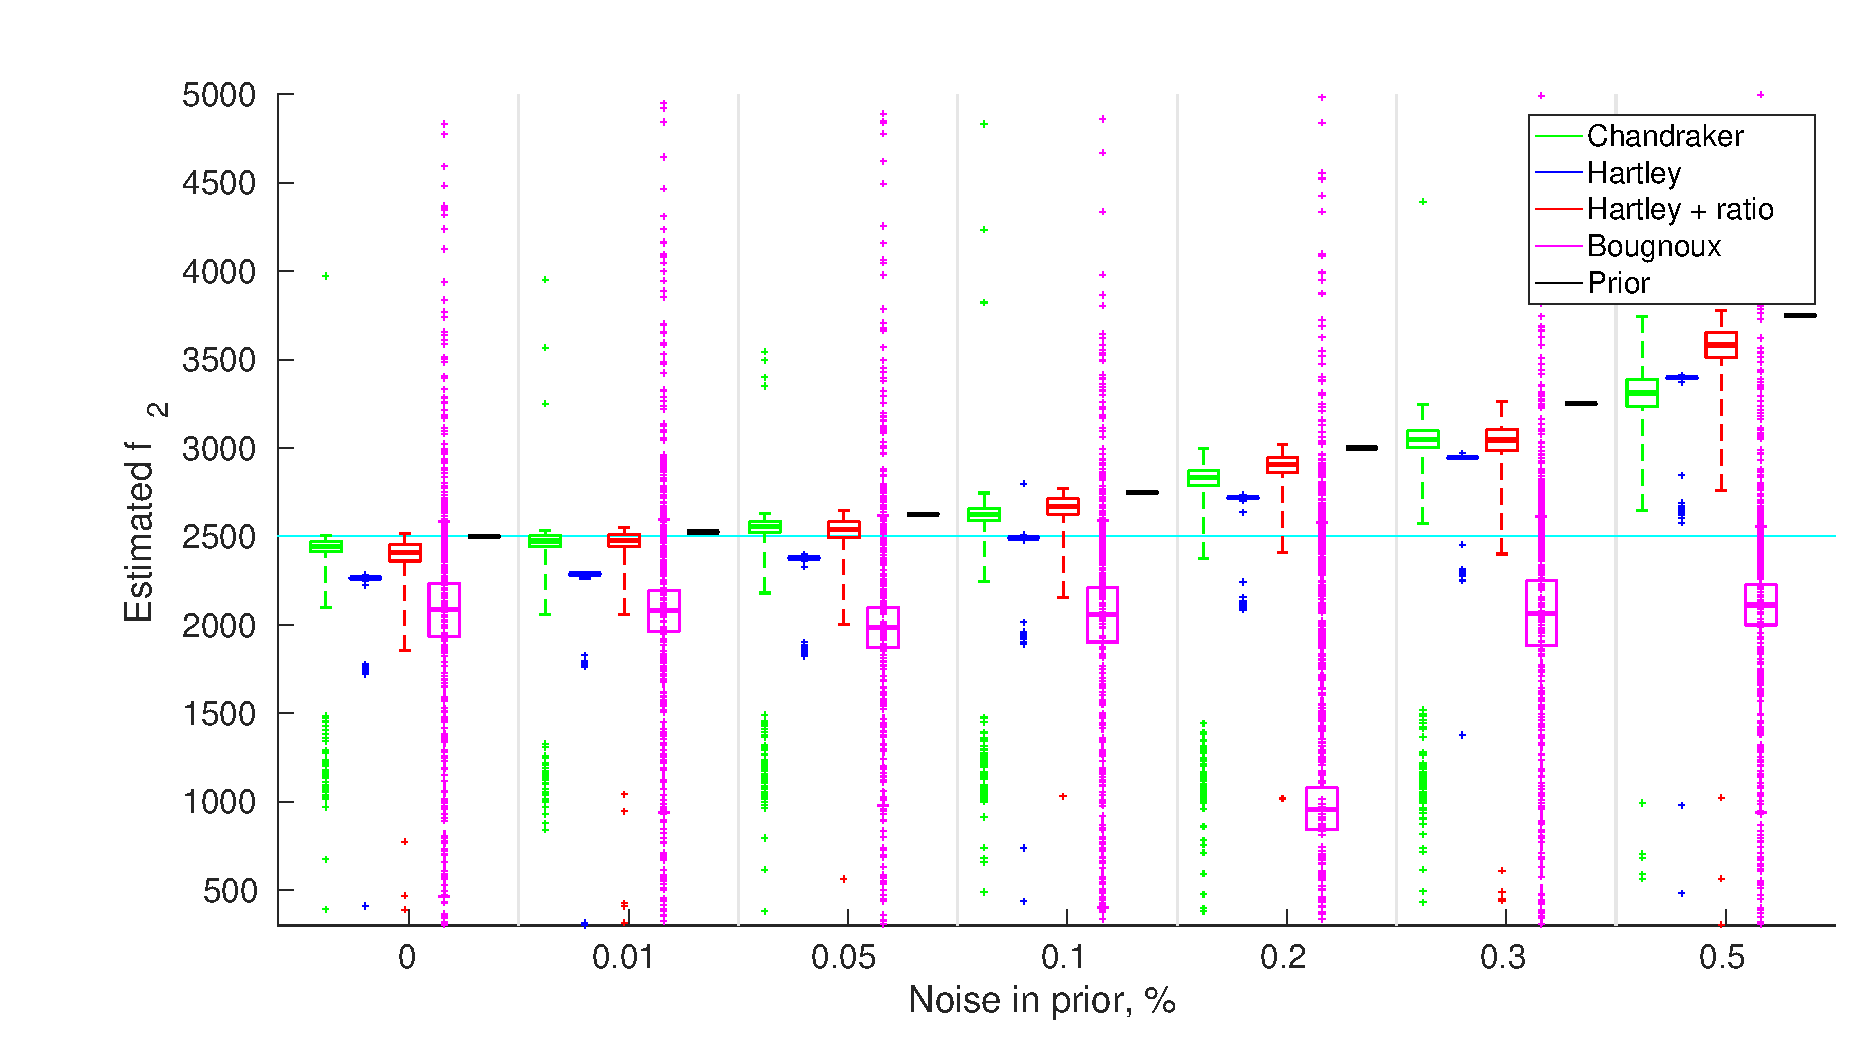
\includegraphics[width=\linewidth]{opt_comp_f2.eps}
    \caption[Comparison of the focal length methods. f1]{A comparison of the methods for computing focal lengths from point correspondences.  The ground truth focal length $f_2$ was 2500 (shown in cyan), and the relative noise (axis $x$) was added to it to produce priors, i. e., the priors were: 2500, 2525, 2625, 2750, 3000, 3250, 3750.}
    \label{opt_comp_f2}
  \end{center}
\end{figure}

\section{Conclusions}
We conclude that the fact that focal length ratio $r= f_2\slash f_1$ is robust can be used to construct more efficient algorithms. We show two examples of modifications to existing algorithms where we explicitly use a ratio estimation to improve the accuracy of the focal lengths computation. We show that using prior knowledge about focal length considerably bigger amounts of noise could be treated.